\section{Versuchsaufbau/-durchführung}
Der Versuchsaufbau, der sich in allen Teilen der Durchführung nur geringfügig unterscheidet, ist in Abbildung \ref{fig: aufbau} einzusehen. %Abildung abgebildet
Die Form der Generatorspannung $U\ua{G}$ wird dem jeweiligen Abschnitt der Messung angepasst. Bei dem Zweikanal-Oszilloskop handelt es sich um ein %Satz kürzen
digitales Gerät, dessen Measure-Einstellung zur Ausmessung von Spannungsamplituden und Zeitdifferenzen verwendet wird. Diese geben Aufschluss über
die in der Theorie erwähnten Zusammenhänge zwischen Generator- und Kondensatorspannung.
\begin{figure}
  \centering
  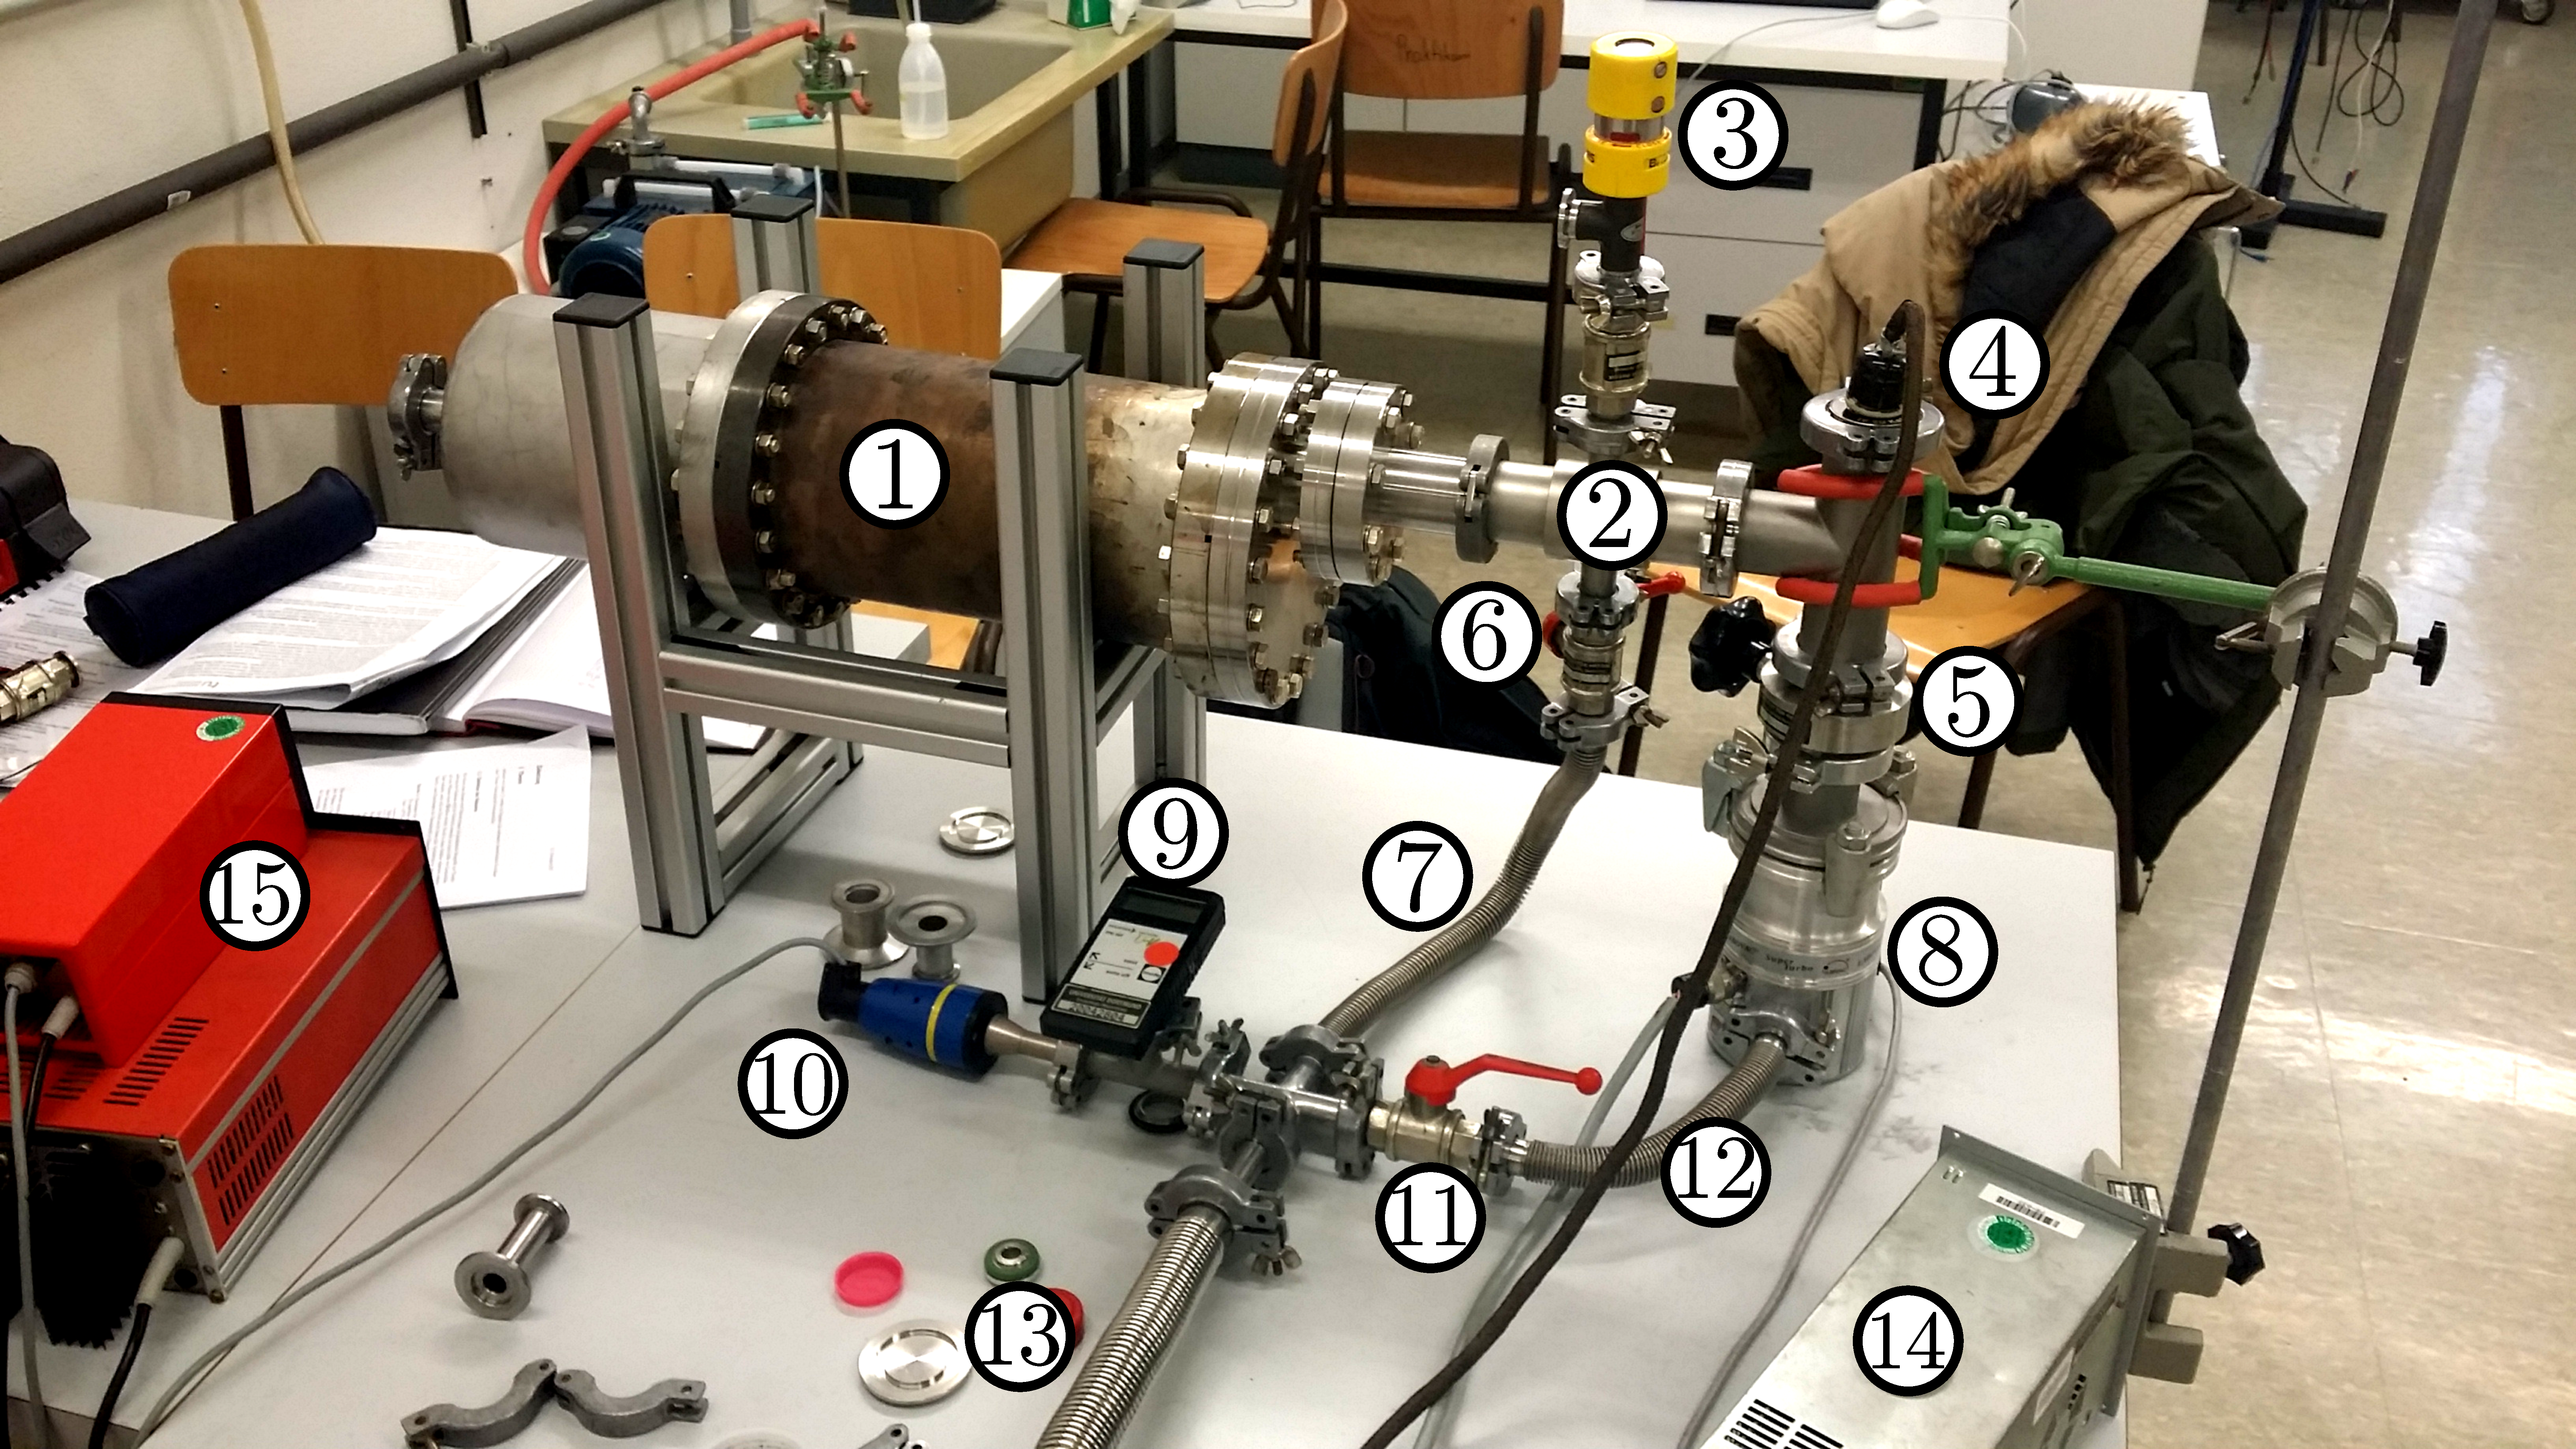
\includegraphics[width = \textwidth]{pics/aufbau.png}
  \caption{Aufbau zur Untersuchung des Relaxationsverhaltens eines RC-Gliedes.}
  \label{fig: aufbau}
\end{figure}

\subsection{Bestimmung der Zeitkonstante RC}
Um die Zeitkonstante $RC$ zu bestimmen, wird am Generator G in Abbildung \ref{fig: aufbau} eine Rechteckspannung eingestellt.
Am Oszilloskop werden die Generatorspannung $U\ua{G}$ und die Entladekurve $U\ua{C}$ des Kondensators beobachtet und mittels eines Screenshots %Screenshot, kein thermodruck
dokumentiert.

\subsection{Untersuchung der Frequenzabhängigkeit von Phasenverschiebung und Amplitude}
Am Generator wird eine Sinusspannung eingestellt, deren Frequenz varriert wird (Frequenzbereich: $\sim\SI{10}{\hertz}<\nu<\, \sim\SI{5000}{\hertz}$). %besser 5000
Mittels der Measure-Einstellung des digitalen Voltmeters werden die Periodendauer $b$ der
Generatorspannung $U\ua{G}$, sowie deren zeitliche Verschiebung $a$ zur Kondensatorspannung $U\ua{C}$ ausgemessen. Diese beiden Werte ermöglichen gemäß
\begin{equation}
  \varphi = \frac{a}{b}2\pi
  \label{eq:phasenverschiebung}
\end{equation}
die Bestimmung der Phasenverschiebung. Darüber hinaus werden für die selben Frequenzen die Amplituden der beiden Spannungen mittels des Oszilloskops
bestimmt.

\subsection{Untersuchung der Integrator-Eigenschaft des RC-Kreises}
Für diese Messung wird am Generator eine Frequenz von \textbf{hier noch die rchtige Frequenz einfügen}$\SI{}{\hertz}$ eingestellt, die dem in der Theorie erwähnten Grenzfall $\omega \gg RC^{-1}$ genügt. %hier noch den richtigen Frequenzbereich einfügen
Für eine Rechteck-, Sinus- und Dreiecksspannung wird
jeweils ein Screenshot des auf dem Oszillosgraphen erkennbaren Bildes erstellt. Dieser ermöglicht eine qualitative Untersuchung der %Screenshot
Integrator-Eigenschaft des RC-Kreises. %eines RC-Kreises
